\chapter{Repetition Code}
\label{sec:classical_repetition_code}

Suppose a noisy channel in which, with probability $p$, a bit that passes through flips. This implies that we will only get the correct information with probability $(1 - p)$. We can obtain better results by encoding the information. In this case, suppose we are taking a single bit of information and encoding it with three additional bits. A particular aspect of this model to consider is that every bit in that sequence holds the same amount of information. This is a strictly classical concept called \textit{redundancy}.

\begin{figure}[H]
\centering
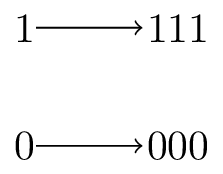
\includegraphics[width=0.5\linewidth]{files/01_repetition_code-83776af5f392140f3fd27f74c40e0424.png}
\caption[]{Representation of the repetition code. This image was inspired by the book \citep{Nielsen2010}. It shows that each bit is represented by three bits---a strictly classical form of redundancy.}
\label{img_1}
\end{figure}

After passing through the channel, we obtain a new bit string. For the sake of example, let's call it $S_n$. This bit string could be the original one or any other combination of the three bits, depending on how many times an error occurred. Decoding is where we gain most of the benefits of using a code in the first place, and in this example there are two primary decoding methods to improve fidelity:

\begin{enumerate}
\item We could build a majority-vote system, meaning we interpret the bit string as representing bit 0 if the majority of elements are 0, and similarly for 1.
\item The other decoding method is to check if two bits are equal. This detects that an error occurred and indicates how to correct it. In this particular case, you can compare the first and second bits, and the first and third bits.
\end{enumerate}

These two systems work essentially the same way in classical computing theory. However, the first method cannot be directly translated into quantum computing because it requires measuring each bit independently. Therefore, we will focus on the second option for the decoding process so that a parallel can be drawn with the quantum equivalent of this code.

For ease of understanding, consider the case where the decoding process receives the bit string 010. In that scenario, the decoding process would indicate that the first and second bits are different and that the first and third bits are equal, implying that the second bit was the source of the error.

However, that could be the wrong assumption; it is possible that the first and third bits were actually the ones affected by the error. This indistinguishability between the two possibilities indicates that this code works only if an error occurs in at most one bit. Therefore, the probability of an error with this code is

\begin{equation}
p^3 + 3p^2(1 - p) = 3p^2 - 2p^3.
\end{equation}

\begin{figure}[H]
\centering
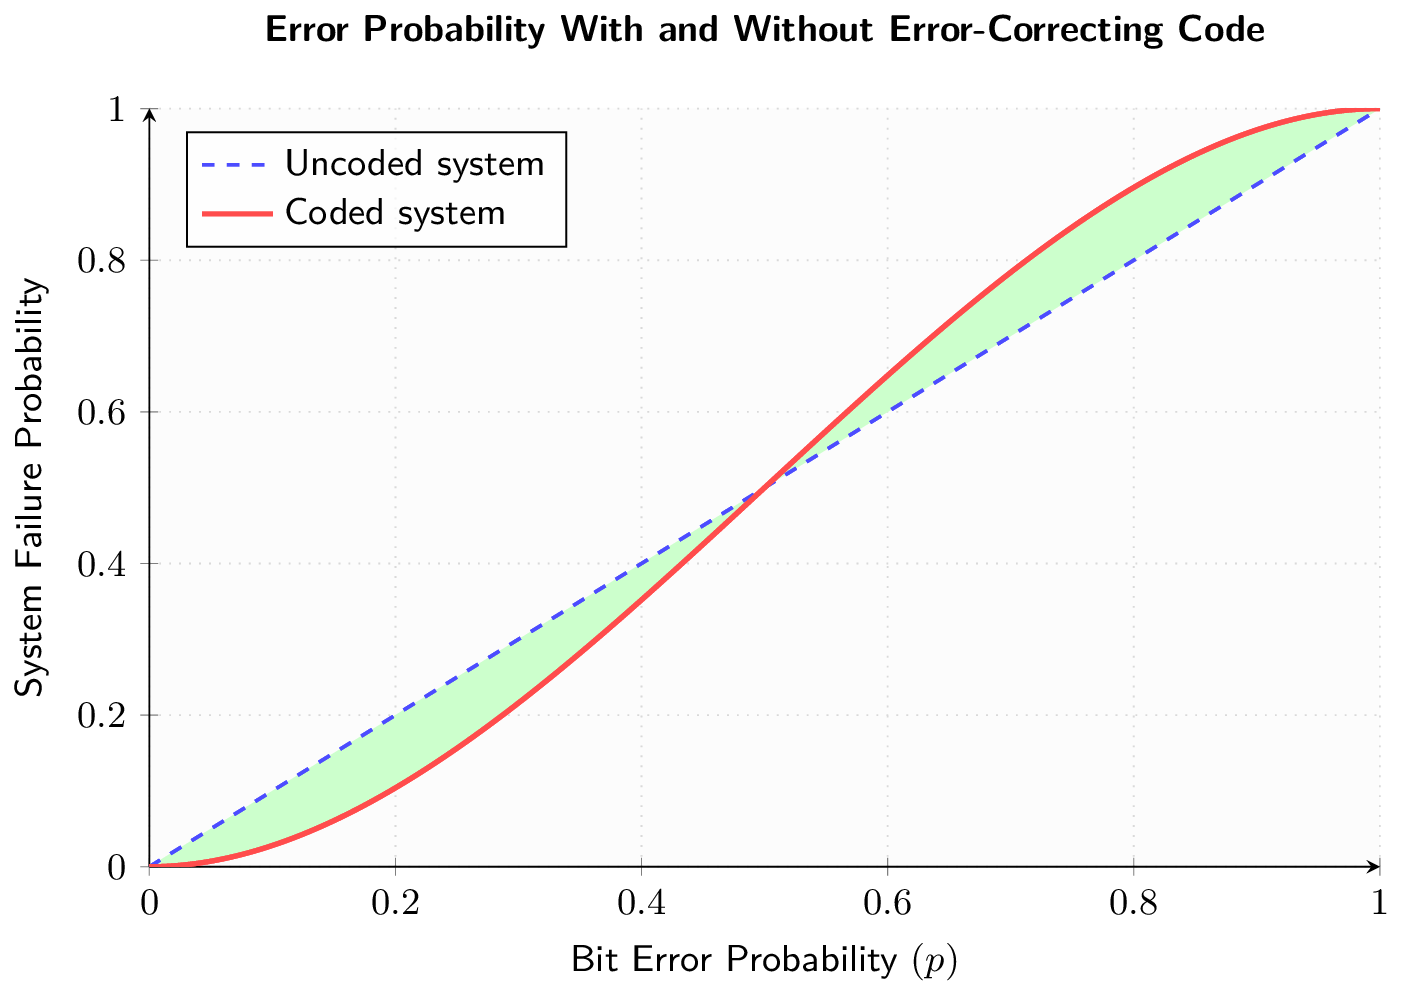
\includegraphics[width=0.7\linewidth]{files/02_comparison-2d9e0d455373d64bb1d46105fb84b631.png}
\caption[]{Comparison of the probability of error for a bit transmitted through the channel with and without the code. The dashed blue line represents the unprotected bit, whose error probability is linear. The red line represents the coded system, which performs better when the error probability is less than 50\%.}
\label{img_2}
\end{figure}

Note that without coding, the probability of failure is $p$. Therefore, this code is only helpful if $3p^2 - 2p^3 \le p$, which holds only when $p \le \frac{1}{2}$. One can actually increase the number of bits used to encode the same amount of information and obtain different thresholds of usefulness---there has been extensive work in classical coding theory on this. However, the core idea of encoding information is already captured by this example.

%  TODO: Debo agregar una sección haciendo los calculos para un sistema de votación arbitrario para $n$ bits? Podria ser interesante

